\documentclass[a4paper,11pt]{report}

\usepackage{amsmath}
\usepackage{fullpage}
\usepackage{tikz}

\usepackage{bussproofs}
\usepackage{mathpartir}
\usepackage{prooftrees}
\usepackage{color}

\makeatletter
\pgfmathdeclarefunction{alpha}{1}{%
  \pgfmathint@{#1}%
  \edef\pgfmathresult{\pgffor@alpha{\pgfmathresult}}%
}

\author{Sylvain Julmy}
\date{\today}

\setlength{\parindent}{0pt}

\begin{document}

\begin{center}
  \Large{
    Mathematical Methods for Computer Science 1\
    Fall 2017
  }
  \noindent\makebox[\linewidth]{\rule{\linewidth}{0.4pt}}

  Series 5
  \vspace*{1.4cm}

  Sylvain Julmy
  
  \noindent\makebox[\linewidth]{\rule{\linewidth}{0.4pt}}
\end{center}

\section*{\texttt{1}}
\subsection*{a)}

Note : the labels are here for visual purpose, the trees are unlabelled.

\begin{minipage}{0.3\textwidth}
\begin{forest}
  [a  [b  [c  [d  [e  [f]  ]  ]  ]  ]  ]
\end{forest}
\end{minipage}
\begin{minipage}{0.3\textwidth}
\begin{forest}
  [a  [b  [c  [d  [e] [f]  ]  ]  ] ]
\end{forest}
\end{minipage}
\begin{minipage}{0.3\textwidth}
\begin{forest}
  [a  [b  [c  [d]  [e]  [f] ]  ]  ]
\end{forest}
\end{minipage}

\begin{minipage}{0.3\textwidth}
\begin{forest}
  [a [b] [c] [d [e] [f]]]  
\end{forest}
\end{minipage}
\begin{minipage}{0.3\textwidth}
\begin{forest}
  [a  [b]  [c]  [d]  [e]  [f]  ]
\end{forest}
\end{minipage}
\begin{minipage}{0.3\textwidth}
\begin{forest}
  [a [b [e]] [c [f]] [d]]
\end{forest}
\end{minipage}

\subsection*{b)}

We use the following lemma : in every tree, there is at least two leaf (proven
during the course). We denote $v$ the vertices with degree $d$. We consider the
sub-tree of $d$ which are all tree (of at least one element). If there is only
one element in the sub-tree, there is one leaf. If there is multiple element in
the sub-tree, there is at least $2$ leaves in the sub-tree and we remove $1$
because the leaves could be connected to $v$. So every sub-tree adjacent to $v$
hold at least $1$ leaves, because there is $d$ subtree, there is at least $d$
leaves in total in the tree.

\section*{\texttt{2}}

\subsection*{a)}

In the graph $P_{m,n} = (V,E)$, there is $|V| = m * n$. In order to obtain the maximal
number of removable edges, such that the graph remains connected, we could
contruct a tree $T = (V',E')$ where $V' = V$ and $E' \subset E$. We know
that $|V'| = |E'| + 1$, so the number of removable edges from $E$ is $|E| -
(|E'| + 1)$, where $|E| = n(m-1) + m(n-1) = mn - n + mn - m = 2mn - m - n $ and
$|E'| = |V'| - 1 = |V| - 1 = mn - 1$. Finally we have the number of removable
vertices : $2mn - m - n - (mn - 1 + 1) = mn - m - n$.

\subsection*{b)}

We denote the vertex for the king $K$, and $deg(K)= 4$. From ``10 of his male
descendants had $3$ sons each'', we know that there is $10$ vertices of degree
$4$ each, and from ``15 had 2 sons'', we know that there is $15$ vertices of
degree $3$ each.

We also know, from theorem, that $|V| = |E| + 1$ and $\sum_{v \in V} deg(v) = 2|E|$.

Then, we have $4 + (10 * 4) + (15 * 3) + x = 2|E|$. Where $x$ is the number of
childless sons of degree $1$. Then, the number of vertices $|V|$ is $|V| = 1 +
10 + 15 + x$, $1$ for the king and $x$ for the number of childless sons.
Finally, using the formula $|V| = |E| + 1$, we have

\begin{align*}
  |V| &= |E| + 1 \\
  |V| - 1 &= |E| \\
  1 + 10 + 15 - 1 + x &= \frac{4 + (10*4) + (15*3) + x}{2}\\
  25 + x &=  \frac{89 + x}{2}\\
  x - \frac{x}{2} &= \frac{89}{2} - 25\\
  \frac{x}{2} &=  \frac{89}{2} - 25\\
  x &= 2 (\frac{89}{2} - 25) \\
  x &= 89 - 50 \\
  x &= 39
\end{align*}

So the number of male descendants is $39 + 10 + 15 = 64$.

\section*{\texttt{3}}

\subsection*{a)}

We assume that $T + e - e^\prime$ also remove and add the corresponding tree otherwise
$T + e - e^\prime$ would not be a tree but a forest.

$T + e - e^\prime$ is a spanning tree, because if $E(G) \setminus E(T) \neq \emptyset$,
that means there is a cycle in $G$ so there is multiple path to go to $e$. If
$E(G) \setminus E(T) = \emptyset$, that means there is no cycle in $G$ so the
graph is already a tree.

\subsection*{b)}

We denote $AB$ the edges which is going from $A$ to $B$.

\begin{center}
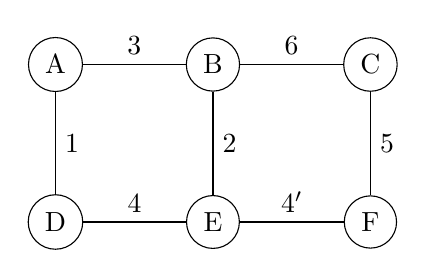
\begin{tikzpicture}
  \node[shape=circle,draw=black] (a) at (0,0) {A};
  \node[shape=circle,draw=black] (b) at (2,0) {B};
  \node[shape=circle,draw=black] (c) at (4,0) {C};
  \node[shape=circle,draw=black] (d) at (0,-2) {D};
  \node[shape=circle,draw=black] (e) at (2,-2) {E};
  \node[shape=circle,draw=black] (f) at (4,-2) {F};
  \draw (a) to node [above] {3}  (b);
  \draw (b) to node [above] {$6$} (c);
  \draw (c) to node [right] {$5$} (f);
  \draw (a) to node [right] {$1$} (d);
  \draw (b) to node [right] {$2$} (e);
  \draw (d) to node [above] {$4$} (e);
  \draw (f) to node [above] {$4^\prime$} (e);
\end{tikzpicture}
\end{center}

\begin{itemize}
\item Order the edges by weight : $e_{sort} = (1,2,3,4,4^\prime,5,6) = (AD,BE,AB,DE,EF,CF,BC)$
\item $E_0 = \emptyset$
\item $E_1 = E_0 \cup \{AD\} = \{AD\}$
\item $E_2 = E_1 \cup \{BE\} = \{AD,BE\}$
\item $E_3 = E_2 \cup \{AB\} = \{AD,BE,AB\}$
\item $E_4 = E_3 = \{AD,BE,AB\}$ because $E = \{AB,BE,DE,AD\}$ has a cycle
\item $E_5 = E_4 \cup \{EF\} = \{AD,BE,AB,EF\}$
\item $E_6 = E_5 \cup \{FC\} = \{AD,BE,AB,EF,CF\}$
\item Stop, because $|E_6| = 5 = |V| - 1$
\end{itemize}

So the minimal spanning tree is $T = \{AD,BE,AB,EF,CF\} = \{1,2,3,4^\prime,5\}$.

\section*{\texttt{4}}

\subsection*{a)}

We denote $AB$ the edges which is going from $A$ to $B$.

\begin{itemize}
\item Order the edges in the non-decreasing order pf their weight : $e_{sort} =
  (6,5,4,4^\prime,3,2,1) = (BC,CF,DE,EF,AB,BE,AD)$
\item Choose an initial vertex $v$ : $v = B$
\item $V_0 = \{v\}, E_0 = \emptyset$
\item $e_k = \{B,E\}, k = 2, V_1 = V_0 \cup \{E\}, E_1 = E_0 \cup \{BE\} = \{BE\}$
\item $e_k = \{B,A\}, k = 3, V_2 = V_1 \cup \{A\} = \{E,A\}, E_2 = E_1 \cup \{BA\} = \{BE,AB\}$
\item $e_k = \{A,D\}, k = 1, V_3 = V_2 \cup \{D\} = \{E,A,D\}, E_3 = E_2 \cup \{AD\} = \{BE,AB,AD\}$
\item $e_k = \{E,F\}, k = 4, V_4 = V_3 \cup \{F\} = \{E,A,D,F\}, E_4 = E_3 \cup \{EF\} = \{BE,AB,AD,EF\}$
\item $e_k = \{F,C\}, k = 5, V_5 = V_4 \cup \{C\} = \{E,A,D,F,C\}, E_5 = E_4
  \cup \{FC\} = \{BE,AB,AD,EF,CF\}$
  \item The algorithm stop because we can't find a $k$, all the vertices of $E$
    are in $E_5$.
\end{itemize}

\subsection*{b)}

$T = (V_i,E_i)$ is a spanning of $G = (V,E)$, because each vertices has been
choose from $V$, so we have $V_i = V$. If every vertices from $V$ are not in
$V_i$, it means that there exist a $k$ and the algorithm should not have to
stop. $T$ does not have any cycle, because we only add vertices to $V_i$ (and
corresponding edges to $E_i$) that are not in $V_i$, so having a cycle is
impossible.

\subsection*{c)}

Let $T$ be the spanning tree of $G$ construct with the Jarnik-Prism algorithm,
and $T'$ the known minimal spanning tree of $G$. If $T = T'$, the spanning tree
is minimal. If $T \neq T'$, it means that $w(T) > w(T')$, so, at a certain
moment in the algorithm, $w(T_i)$ would have increase wrongly with an edge that
has been choosen wrongly by the algorithm. Because the algorithm choose the
smallest possible weight at each iteration, this is impossible.

\section*{\texttt{5}}

\begin{center}
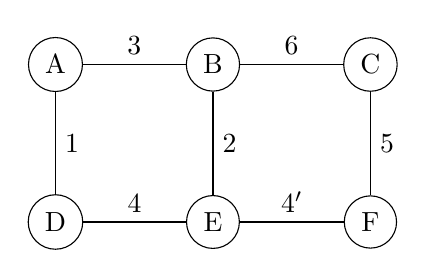
\begin{tikzpicture}
  \node[shape=circle,draw=black] (a) at (0,0) {A};
  \node[shape=circle,draw=black] (b) at (2,0) {B};
  \node[shape=circle,draw=black] (c) at (4,0) {C};
  \node[shape=circle,draw=black] (d) at (0,-2) {D};
  \node[shape=circle,draw=black] (e) at (2,-2) {E};
  \node[shape=circle,draw=black] (f) at (4,-2) {F};
  \draw (a) to node [above] {3}  (b);
  \draw (b) to node [above] {$6$} (c);
  \draw (c) to node [right] {$5$} (f);
  \draw (a) to node [right] {$1$} (d);
  \draw (b) to node [right] {$2$} (e);
  \draw (d) to node [above] {$4$} (e);
  \draw (f) to node [above] {$4^\prime$} (e);
\end{tikzpicture}
\end{center}

We start with $D$.

\begin{table}[h]
\centering
\caption{Dijkstra algorithm application}
\label{my-label}
\begin{tabular}{llllllllll}
\cline{1-7} \cline{9-10}
\multicolumn{1}{|l|}{n} & \multicolumn{1}{l|}{$pd(D)$} & \multicolumn{1}{l|}{$pd(A)$} & \multicolumn{1}{l|}{$pd(B)$} & \multicolumn{1}{l|}{$pd(C)$} & \multicolumn{1}{l|}{$pd(E)$} & \multicolumn{1}{l|}{$pd(F)$} & \multicolumn{1}{l|}{} & \multicolumn{1}{l|}{current} & \multicolumn{1}{l|}{visited set} \\ \cline{1-7} \cline{9-10} 
\multicolumn{1}{|l|}{0} & $0$                          & $\infty$                     & $\infty$                     & $\infty$                     & $\infty$                     & $\infty$                     &                       & $D$                          & $\{\}$                           \\ \cline{1-1}
\multicolumn{1}{|l|}{1} & $0$                          & $1$                          & $\infty$                     & $\infty$                     & $4$                          & $\infty$                     &                       & $D$                          & $\{\}$                           \\ \cline{1-1}
\multicolumn{1}{|l|}{2} & $0$                          & $1$                          & $4$                          & $\infty$                     & $4$                          & $\infty$                     &                       & $A$                          & $\{D\}$                          \\ \cline{1-1}
\multicolumn{1}{|l|}{3} & $0$                          & $1$                          & $4$                          & $\infty$                     & $4$                          & $8$                          &                       & $E$                          & $\{D,A\}$                        \\ \cline{1-1}
\multicolumn{1}{|l|}{4} & $0$                          & $1$                          & $4$                          & $10$                         & $4$                          & $8$                          &                       & $B$                          & $\{D,A,E\}$                      \\ \cline{1-1}
\multicolumn{1}{|l|}{5} & $0$                          & $1$                          & $4$                          & $10$                         & $4$                          & $8$                          &                       & $F$                          & $\{D,A,E,B\}$                    \\ \cline{1-1}
\multicolumn{1}{|l|}{6} & $0$                          & $1$                          & $4$                          & $10$                         & $4$                          & $8$                          &                       & $C$                          & $\{D,A,E,B,F\}$                  \\ \cline{1-1}
                        &                              &                              &                              &                              &                              &                              &                       &                              & $\{D,A,E,B,F,C\}$               
\end{tabular}
\end{table}

The shortest path from $D$ to $C$ is $D \rightarrow A \rightarrow B \rightarrow
C$ with a total weight of $1+3+6 = 10$.

\section*{\texttt{6}}

We use the fact that in every tree $T = (V,E)$, $|V| = |E| + 1$, that implies
$|V| - 1 = |E|$, and in every graph $G = (V,E)$, $\sum_{v \in V} deg(v) =
2*|E|$. So we have :

\begin{align*}
  & |E| = |V| - 1 \\
  & 2*|E| = 2(|V| - 1) \\
  & |V| = n \\
  & \sum_{v \in V} deg(v) = 2*|E|
\end{align*}

Finally we conclude that

\begin{align*}
  \sum_{v \in V} deg(v) &= 2*|E| \\
  \sum_{v \in V} deg(v) &= 2*(|V| - 1) \\
  \sum_{v \in V} deg(v) &= 2*(n - 1) \\
  \sum_{v \in V} deg(v) &= 2n - 2 \\
  \sum_{i=0}^n d_i &= 2n - 2
\end{align*}

\end{document}